\subsection{Memory stage} 
\label{section:stage_mem}

The memory stage comes right after execute and is resposible for all accesses
to the data memory. In our design the data memory is located externally and 
the actual implementation of the stage simply drives a few signals out of 
the processor core. Logically, however, the data memory can be drawn within the
stage as in figure~\ref{fig:stage_mem}.

\begin{figure}[h]
        \centering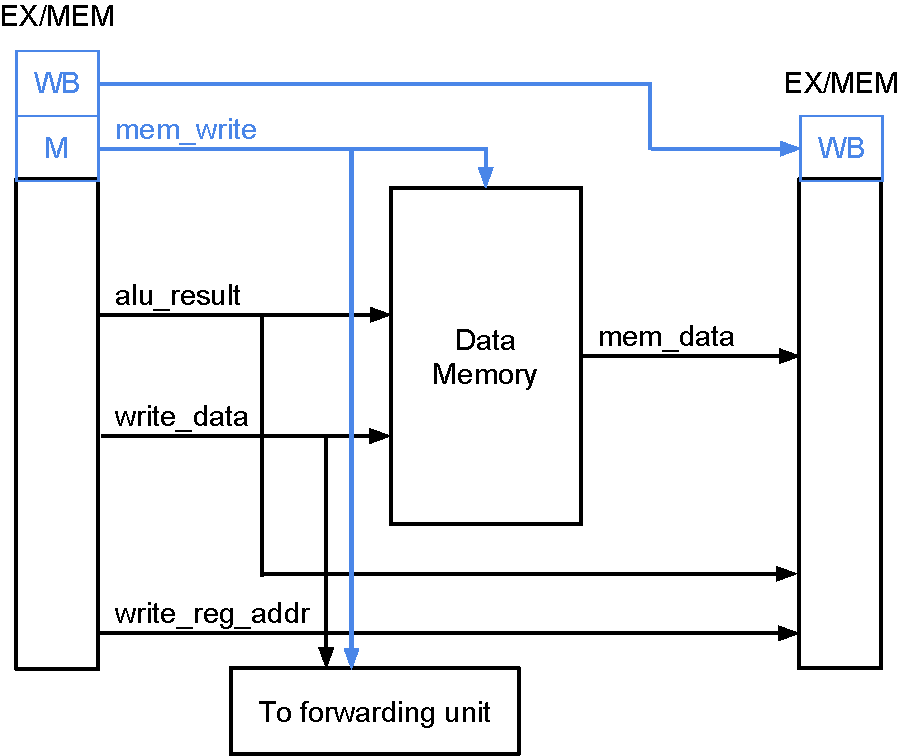
\includegraphics[scale=0.5]{figures/stage_mem}
        \caption{The stage\_mem architecture}
        \label{fig:stage_mem}
\end{figure}

The main point in this stage is that the alu result drives the memory read and
write address. This is done because load and store word uses the alu to calulcate
the actual memory offset. The memory data input is connected to the \emph{write\_data}
signal in the pipeline register. During a store this is filled with the value of
register 2 by execute. Whether or not the data memory is to be written to, is 
controlled by a signal in the pipeline register.

To the next pipeline register this stage sends the alu result aswell as whatever
the output of the data memory was. The decision whether the alu or data memory 
result is to be forwarded to the register file is handled by the write back stage.
